\documentclass[11pt,a4paper]{article}
\usepackage[utf8]{inputenc}
\usepackage[T1]{fontenc}
\usepackage{geometry}
\geometry{margin=2.5cm}
\usepackage{tikz}
\usetikzlibrary{arrows.meta, positioning, fit, backgrounds, shapes.geometric, calc}
\usepackage{listings}
\usepackage{xcolor}
\usepackage{booktabs}
\usepackage{hyperref}
\usepackage{enumitem}
\usepackage{amsmath}
\usepackage{titlesec}
\usepackage{fancyhdr}

\hypersetup{colorlinks=true, linkcolor=blue!50!black, urlcolor=blue!50!black, citecolor=blue!50!black}

\titleformat{\section}{\normalfont\Large\bfseries}{\thesection}{1em}{}
\titleformat{\subsection}{\normalfont\large\bfseries}{\thesubsection}{1em}{}

\pagestyle{fancy}
\fancyhf{}
\fancyhead[L]{\small Refonte événementielle -- DNN//$^{*}$Tcs}
\fancyhead[R]{\small\thepage}
\renewcommand{\headrulewidth}{0.4pt}

\definecolor{boxblue}{RGB}{224,236,248}
\definecolor{boxred}{RGB}{250,224,224}
\definecolor{boxgreen}{RGB}{224,248,232}
\definecolor{boxpurple}{RGB}{237,228,247}
\definecolor{codebg}{RGB}{245,245,245}

\lstdefinestyle{python}{
  backgroundcolor=\color{codebg},
  basicstyle=\ttfamily\footnotesize,
  keywordstyle=\color{blue!70!black}\bfseries,
  commentstyle=\color{green!40!black}\itshape,
  stringstyle=\color{orange!70!black},
  showstringspaces=false,
  breaklines=true,
  frame=single,
  rulecolor=\color{gray!40},
  language=Python,
  tabsize=4,
  numbers=left,
  numberstyle=\tiny\color{gray}
}

\usepackage[most]{tcolorbox}

\newtcolorbox{probleme}[1]{
  colback=boxred, colframe=red!40!black, boxrule=0.4pt, arc=2pt,
  title={Limite observée --- #1}, fonttitle=\bfseries\small,
  coltitle=black, colbacktitle=red!25, left=6pt, right=6pt, top=3pt, bottom=3pt
}

\newtcolorbox{correction}[1]{
  colback=boxgreen, colframe=green!30!black, boxrule=0.4pt, arc=2pt,
  title={Traitement retenu --- #1}, fonttitle=\bfseries\small,
  coltitle=black, colbacktitle=green!25, left=6pt, right=6pt, top=3pt, bottom=3pt
}

\newtcolorbox{principe}[1]{
  colback=boxpurple, colframe=violet!40!black, boxrule=0.4pt, arc=2pt,
  title={#1}, fonttitle=\bfseries\small,
  coltitle=black, colbacktitle=violet!20, left=6pt, right=6pt, top=3pt, bottom=3pt
}

\title{\bfseries Une architecture événementielle pour le système\\[2pt]
\textit{Parallel Collective Tiny Deep Learning} (DNN//$^{*}$Tcs)\\[6pt]
\large Modélisation C4 centrée flux et log d'événements}
\author{Proposition alternative fondée sur le traitement de flux}
\date{}

\begin{document}
\maketitle
\thispagestyle{fancy}

\begin{abstract}
\noindent
L'article de Helaoui et Bahroun décrit un système de détection et de reconnaissance
(visage, émotion, genre, objet) qui combine une version cliente allégée, une version serveur
précise et des micro-contrôleurs connectés (« objets Tiny ») dont les mesures servent de
vérité terrain pour corriger les classifications. Le déploiement réel décrit dans l'article
reste toutefois un multiprocessing sur une seule machine, sans véritable réseau distribué.
Ce document propose une architecture cible différente de la lecture microservices/REST
habituelle : une architecture \textbf{événementielle}, où chaque détection, chaque mesure Tiny
et chaque décision est un \textbf{événement immuable} publié sur un journal partagé, et où la
fusion entre versions de modèles est réalisée par un \textbf{processeur de flux} plutôt que par
un service interrogé de manière synchrone. Cette lecture répond aux mêmes exigences que
l'article original (temps réel, robustesse aux erreurs de classification, intégration des
données Tiny) mais élimine par construction plusieurs faiblesses structurelles : couplage entre
émetteur et récepteur, absence de rejouabilité, et incapacité à corriger une décision déjà
émise lorsqu'une donnée Tiny arrive en retard.
\end{abstract}

\tableofcontents

% ============================================================
\section{Introduction}
% ============================================================

Le système DNN//$^{*}$Tcs répond à un besoin de décision temps réel à partir de plusieurs
sources hétérogènes : un ou plusieurs modèles de vision embarqués sur le client, des modèles
plus lourds exécutés côté serveur, et des mesures directes transmises par des objets connectés.
La question centrale n'est donc pas seulement « comment répartir le calcul sur plusieurs
processeurs ? » --- déjà traitée en détail par les auteurs via les lois d'Amdahl et de Brent
--- mais « comment combiner, en continu, des observations qui n'arrivent jamais toutes en même
temps, sans perdre celles qui arrivent en retard ni bloquer celles qui sont déjà disponibles ? ».
C'est une question de \textbf{traitement de flux}, pas seulement de calcul parallèle. Ce
document propose une lecture du problème sous cet angle, avec un log d'événements comme
source de vérité unique et une série de vues dérivées (projections) qui répondent chacune à un
besoin précis : afficher la dernière décision, corriger une décision passée, ou rejouer
l'historique pour audit.

% ============================================================
\section{Ce que l'architecture doit résoudre}
% ============================================================

\subsection{Nature du problème}

Trois familles d'événements alimentent le système, à des rythmes et des degrés de confiance
différents :

\begin{itemize}[leftmargin=1.2cm]
  \item des \textbf{détections de modèles embarqués}, fréquentes, rapides, peu fiables
  individuellement (\emph{lite version} de l'article) ;
  \item des \textbf{détections de modèles serveur}, plus rares dans le temps réel strict mais
  plus précises, arrivant avec un léger délai réseau ;
  \item des \textbf{mesures d'objets connectés}, arrivant de façon irrégulière, parfois
  après la décision qu'elles auraient dû influencer.
\end{itemize}

\begin{probleme}{Le temps réel n'est pas la simultanéité}
Une architecture qui exige que toutes les sources répondent avant de décider (comme un appel
RPC synchrone qui attendrait chaque service) reproduit artificiellement une contrainte de
synchronisation que le problème lui-même n'impose pas : rien n'empêche de publier une première
décision provisoire, puis de la corriger dès qu'une mesure plus fiable arrive.
\end{probleme}

\begin{probleme}{La perte d'historique empêche l'audit et le rejeu}
Un système qui ne conserve que le dernier résultat de chaque service ne permet ni de rejouer
une séquence pour diagnostiquer une erreur de classification, ni d'entraîner de nouveaux
modèles sur les décisions passées, ni de corriger une décision après coup lorsqu'une donnée
Tiny arrive en retard --- exactement le scénario mis en évidence dans les figures de confusion
de l'article, où les objets Tiny corrigent des faux positifs de YOLOv8 après plusieurs images.
\end{probleme}

\begin{probleme}{Le couplage émetteur/récepteur limite l'évolutivité}
Si chaque service de détection doit connaître à l'avance le service de fusion pour lui envoyer
son résultat, ajouter un cinquième modèle (une nouvelle version de CNN, par exemple) impose de
modifier le service de fusion. Un flux découplé, où les producteurs publient sans connaître les
consommateurs, permet d'ajouter un nouveau modèle sans toucher au reste du système.
\end{probleme}

% ============================================================
\section{Principes de la solution événementielle}
% ============================================================

\begin{principe}{Principe 1 --- Le journal d'événements est la seule source de vérité}
Aucun service ne détient d'état interne faisant foi. Toute détection, toute mesure Tiny et
toute décision de fusion est un événement horodaté et immuable, publié une fois pour toutes
sur un journal partagé (\emph{event log}). Les services qui consomment ce journal peuvent être
arrêtés et redémarrés sans perte : ils reconstruisent leur état en rejouant le journal.
\end{principe}

\begin{principe}{Principe 2 --- La décision est une vue dérivée, jamais un appel bloquant}
Il n'existe pas de service « Ensemble » interrogé de façon synchrone. La décision consolidée
est une \textbf{projection} calculée en continu par un processeur de flux qui observe le
journal et met à jour une vue matérialisée à chaque nouvel événement pertinent. Consulter la
décision revient à lire cette vue, jamais à attendre une réponse.
\end{principe}

\begin{principe}{Principe 3 --- Toute décision est révisable}
Puisque les événements sont immuables et horodatés, une mesure Tiny arrivant après une première
décision ne \emph{remplace} pas silencieusement cette décision : elle génère un nouvel
événement de \textbf{révision}, explicitement lié à la décision initiale. Le client peut choisir
d'afficher la dernière révision ou de conserver l'historique des révisions selon son besoin.
\end{principe}

\begin{principe}{Principe 4 --- Les producteurs ignorent les consommateurs}
Un modèle de détection publie ses résultats sur un sujet (\emph{topic}) du journal sans savoir
qui les consomme. Ajouter, retirer ou remplacer un modèle ne nécessite de modifier ni les
producteurs existants ni les consommateurs existants, à la différence d'un appel direct entre
composants.
\end{principe}

% ============================================================
\section{Modélisation C4 de la solution événementielle}
% ============================================================

\subsection{Niveau 1 --- Diagramme de contexte}

Le système consomme un flux vidéo continu et des mesures d'objets connectés, et produit un flux
de décisions consultable en continu --- plutôt qu'une réponse ponctuelle à une requête.

\begin{center}
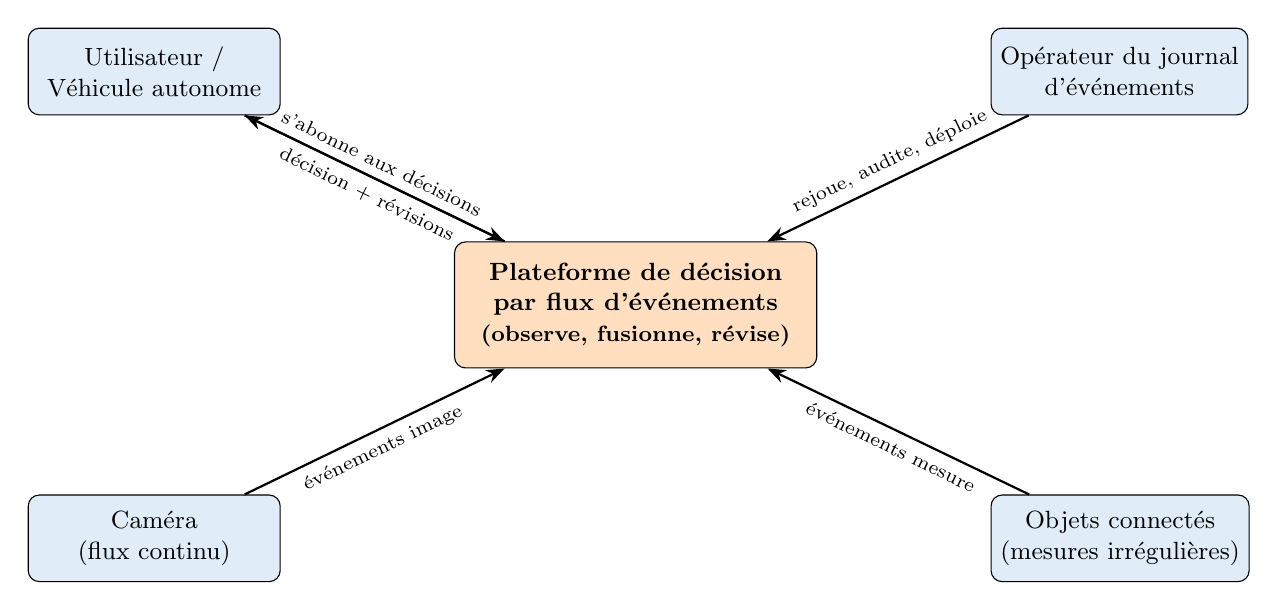
\begin{tikzpicture}[
  node distance=1.6cm and 2.2cm,
  actor/.style={draw, rounded corners, fill=boxblue, minimum width=3.2cm, minimum height=1.1cm, align=center, font=\small},
  sys/.style={draw, rounded corners, fill=orange!25, minimum width=4.6cm, minimum height=1.6cm, align=center, font=\small\bfseries},
  arr/.style={-Stealth, thick}
]
\node[sys] (sys) {Plateforme de décision\\par flux d'événements\\\footnotesize (observe, fusionne, révise)};
\node[actor, above left=of sys] (user) {Utilisateur /\\Véhicule autonome};
\node[actor, above right=of sys] (admin) {Opérateur du journal\\d'événements};
\node[actor, below left=of sys] (cam) {Caméra\\(flux continu)};
\node[actor, below right=of sys] (iot) {Objets connectés\\(mesures irrégulières)};

\draw[arr] (user) -- node[above, sloped, font=\scriptsize]{s'abonne aux décisions} (sys);
\draw[arr] (sys) -- node[below, sloped, font=\scriptsize]{décision + révisions} (user);
\draw[arr] (admin) -- node[above, sloped, font=\scriptsize]{rejoue, audite, déploie} (sys);
\draw[arr] (cam) -- node[below, sloped, font=\scriptsize]{événements image} (sys);
\draw[arr] (iot) -- node[below, sloped, font=\scriptsize]{événements mesure} (sys);
\end{tikzpicture}
\end{center}

\subsection{Niveau 2 --- Diagramme de conteneurs}

Il n'y a plus de séparation « synchrone / asynchrone » à gérer explicitement : \emph{tout}
transite par le journal. La distinction pertinente devient celle entre \textbf{producteurs}
d'événements, \textbf{journal}, \textbf{processeurs de flux} et \textbf{projections}
consultables.

\begin{center}
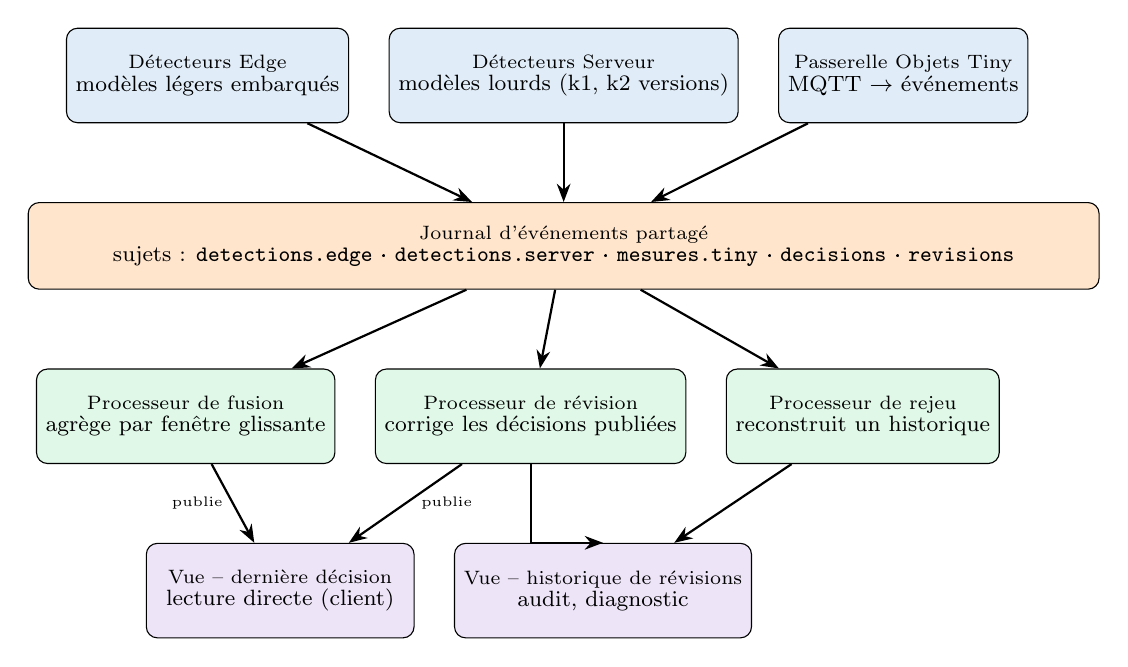
\begin{tikzpicture}[
  node distance=0.85cm and 0.9cm,
  cont/.style={draw, rounded corners, fill=boxblue, minimum width=3.0cm, minimum height=1.2cm, align=center, font=\scriptsize},
  contj/.style={draw, rounded corners, fill=orange!20, minimum width=13.6cm, minimum height=1.1cm, align=center, font=\scriptsize},
  contp/.style={draw, rounded corners, fill=boxgreen, minimum width=3.4cm, minimum height=1.2cm, align=center, font=\scriptsize},
  contv/.style={draw, rounded corners, fill=boxpurple, minimum width=3.4cm, minimum height=1.2cm, align=center, font=\scriptsize},
  flow/.style={-Stealth, thick}
]

% Producers row
\node[cont] (edge) {Détecteurs Edge\\\footnotesize modèles légers embarqués};
\node[cont, right=0.5cm of edge] (srv) {Détecteurs Serveur\\\footnotesize modèles lourds (k1, k2 versions)};
\node[cont, right=0.5cm of srv] (tiny) {Passerelle Objets Tiny\\\footnotesize MQTT $\to$ événements};

% Journal
\node[contj, below=1.0cm of srv] (log) {Journal d'événements partagé\\\footnotesize sujets : \texttt{detections.edge} · \texttt{detections.server} · \texttt{mesures.tiny} · \texttt{decisions} · \texttt{revisions}};

% Stream processors
\node[contp, below=1.0cm of log, xshift=-4.8cm] (fusionproc) {Processeur de fusion\\\footnotesize agrège par fenêtre glissante};
\node[contp, right=0.5cm of fusionproc] (revproc) {Processeur de révision\\\footnotesize corrige les décisions publiées};
\node[contp, right=0.5cm of revproc] (auditproc) {Processeur de rejeu\\\footnotesize reconstruit un historique};

% Projections
\node[contv, below=1.0cm of fusionproc, xshift=1.2cm] (viewlast) {Vue -- dernière décision\\\footnotesize lecture directe (client)};
\node[contv, right=0.5cm of viewlast] (viewhist) {Vue -- historique de révisions\\\footnotesize audit, diagnostic};

\draw[flow] (edge) -- (log);
\draw[flow] (srv) -- (log);
\draw[flow] (tiny) -- (log);

\draw[flow] (log) -- (fusionproc);
\draw[flow] (log) -- (revproc);
\draw[flow] (log) -- (auditproc);

\draw[flow] (fusionproc) -- node[left, font=\tiny]{publie} (viewlast);
\draw[flow] (revproc) -- node[right, font=\tiny, xshift=2pt]{publie} (viewlast);
\draw[flow] (auditproc) -- (viewhist);
\draw[flow] (revproc.south) |- (viewhist.north);

\end{tikzpicture}
\end{center}

\begin{itemize}[leftmargin=1.2cm]
  \item Les \textbf{producteurs} (bleu) ne font qu'écrire des événements sur le journal ; ils
  n'appellent jamais directement un autre composant et n'attendent aucune réponse.
  \item Le \textbf{journal} (orange) conserve tous les événements de façon ordonnée et
  durable, organisés par sujet. C'est la seule dépendance commune à tous les composants.
  \item Les \textbf{processeurs de flux} (vert) lisent le journal en continu et publient à
  leur tour de nouveaux événements (des décisions, des révisions) : ils ne répondent jamais à
  un appelant, ils réagissent à des événements passés.
  \item Les \textbf{vues} (violet) sont des projections consultables directement par
  l'utilisateur, mises à jour en continu par les processeurs.
\end{itemize}

\subsection{Niveau 3 --- Diagramme de composants du processeur de fusion}

C'est le composant qui remplace le service de fusion synchrone : il ne répond pas à une
requête, il réagit à chaque événement entrant en maintenant une fenêtre glissante par
identifiant de scène/objet.

\begin{center}
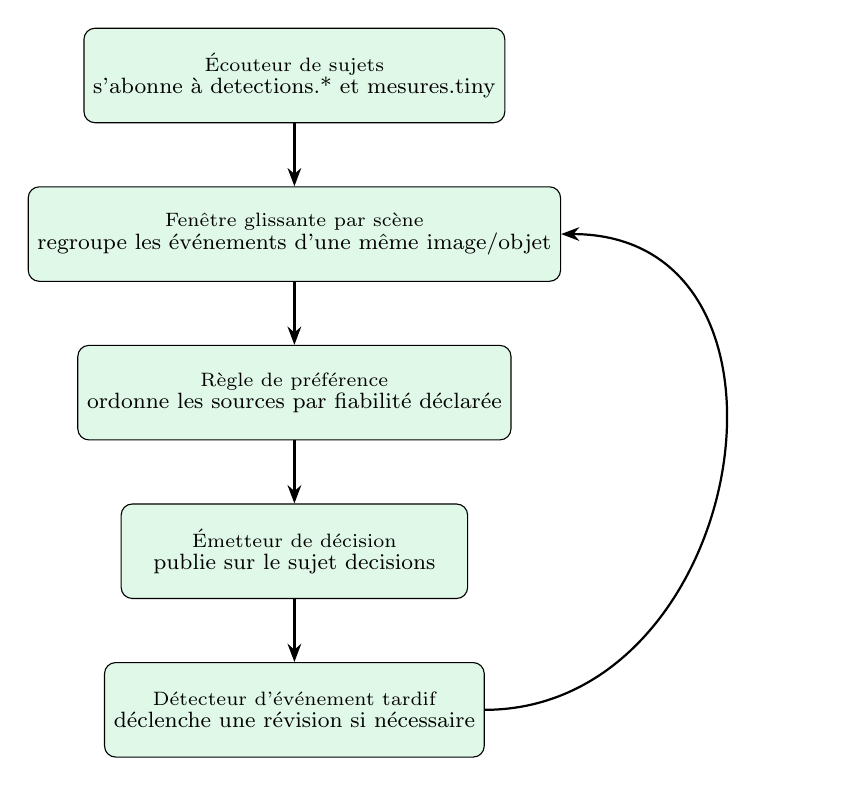
\begin{tikzpicture}[
  node distance=0.8cm and 1.0cm,
  comp/.style={draw, rounded corners, fill=boxgreen, minimum width=4.4cm, minimum height=1.2cm, align=center, font=\scriptsize},
  arr/.style={-Stealth, thick}
]
\node[comp] (listener) {Écouteur de sujets\\\footnotesize s'abonne à detections.* et mesures.tiny};
\node[comp, below=of listener] (window) {Fenêtre glissante par scène\\\footnotesize regroupe les événements d'une même image/objet};
\node[comp, below=of window] (rule) {Règle de préférence\\\footnotesize ordonne les sources par fiabilité déclarée};
\node[comp, below=of rule] (emit) {Émetteur de décision\\\footnotesize publie sur le sujet decisions};
\node[comp, below=of emit] (late) {Détecteur d'événement tardif\\\footnotesize déclenche une révision si nécessaire};

\draw[arr] (listener) -- (window);
\draw[arr] (window) -- (rule);
\draw[arr] (rule) -- (emit);
\draw[arr] (emit) -- (late);
\draw[arr] (late.east) to[out=0,in=0,looseness=1.4] (window.east);
\end{tikzpicture}
\end{center}

Le \textbf{Détecteur d'événement tardif} boucle vers la fenêtre glissante : lorsqu'une mesure
Tiny arrive après qu'une décision a déjà été émise pour la même scène, il ne modifie rien
directement --- il republie l'événement à travers le même chemin, qui produira alors une
\emph{révision} plutôt qu'une première décision. Ce mécanisme répond directement au problème
de la fenêtre d'attente qui, dans une architecture synchrone, obligerait soit à bloquer, soit à
perdre la donnée tardive.

\subsection{Niveau 4 --- Modélisation du code}

La fusion n'est plus un objet \emph{Strategy} instancié par requête, mais une fonction pure de
réduction appliquée à la séquence d'événements observés pour une scène donnée --- une approche
proche du \emph{stream processing} (agrégation par fenêtre, réduction fonctionnelle) plutôt que
de la programmation orientée objet classique.

\begin{center}
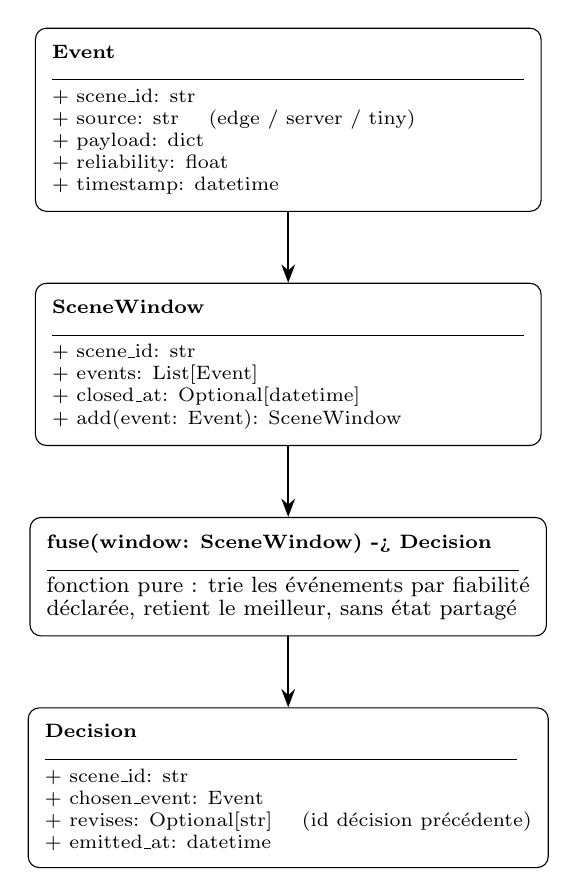
\begin{tikzpicture}[
  node distance=0.9cm and 1.0cm,
  cls/.style={draw, rounded corners, fill=white, minimum width=6.4cm, align=left, font=\scriptsize, inner sep=6pt},
  arr/.style={-Stealth, thick}
]
\node[cls] (event) {\textbf{Event}\\
\rule{6.0cm}{0.3pt}\\
+ scene\_id: str\\
+ source: str \quad (edge / server / tiny)\\
+ payload: dict\\
+ reliability: float\\
+ timestamp: datetime};

\node[cls, below=of event] (window) {\textbf{SceneWindow}\\
\rule{6.0cm}{0.3pt}\\
+ scene\_id: str\\
+ events: List[Event]\\
+ closed\_at: Optional[datetime]\\
+ add(event: Event): SceneWindow};

\node[cls, below=of window] (reduce) {\textbf{fuse(window: SceneWindow) -> Decision}\\
\rule{6.0cm}{0.3pt}\\
\footnotesize fonction pure : trie les événements par fiabilité\\
\footnotesize déclarée, retient le meilleur, sans état partagé};

\node[cls, below=of reduce] (decision) {\textbf{Decision}\\
\rule{6.0cm}{0.3pt}\\
+ scene\_id: str\\
+ chosen\_event: Event\\
+ revises: Optional[str] \quad (id décision précédente)\\
+ emitted\_at: datetime};

\draw[arr] (event) -- (window);
\draw[arr] (window) -- (reduce);
\draw[arr] (reduce) -- (decision);
\end{tikzpicture}
\end{center}

\begin{lstlisting}[style=python, caption={Fusion comme réduction fonctionnelle sur une fenêtre d'événements}]
from dataclasses import dataclass, field
from datetime import datetime
from typing import Optional, List


@dataclass(frozen=True)
class Event:
    """Un evenement est immuable : il n'est jamais modifie apres publication,
    seule une revision publie un nouvel evenement qui en reference un autre."""
    scene_id: str
    source: str            # "edge" | "server" | "tiny"
    payload: dict
    reliability: float      # fiabilite declaree de la source pour ce type d'evenement
    timestamp: datetime


@dataclass
class SceneWindow:
    """Fenetre glissante associee a une scene (une image ou un objet suivi).
    Ne contient aucune logique de decision : un simple accumulateur d'evenements."""
    scene_id: str
    events: List[Event] = field(default_factory=list)
    closed_at: Optional[datetime] = None

    def add(self, event: Event) -> "SceneWindow":
        return SceneWindow(
            scene_id=self.scene_id,
            events=[*self.events, event],
            closed_at=self.closed_at,
        )


@dataclass(frozen=True)
class Decision:
    scene_id: str
    chosen_event: Event
    revises: Optional[str] = None   # id de la decision anterieure, si revision
    emitted_at: datetime = field(default_factory=datetime.utcnow)


def fuse(window: SceneWindow) -> Decision:
    """Fonction pure : aucun etat mutable, aucune dependance a un objet
    instancie au prealable. Remplace le patron Strategy par une simple
    reduction sur la liste d'evenements de la fenetre.

    Regle : la source Tiny, quand elle est presente, prevaut toujours
    (verite terrain) ; sinon on retient l'evenement le plus fiable."""
    tiny_events = [e for e in window.events if e.source == "tiny"]
    if tiny_events:
        chosen = max(tiny_events, key=lambda e: e.timestamp)
    else:
        chosen = max(window.events, key=lambda e: e.reliability)
    return Decision(scene_id=window.scene_id, chosen_event=chosen)


def handle_late_event(previous_decision: Decision, window: SceneWindow) -> Decision:
    """Appelee quand un evenement arrive apres une premiere decision :
    ne modifie jamais la decision existante, publie une revision distincte."""
    new_decision = fuse(window)
    return Decision(
        scene_id=window.scene_id,
        chosen_event=new_decision.chosen_event,
        revises=previous_decision.scene_id,
    )


class FusionProcessor:
    """Consomme le journal d'evenements en continu ; ne repond a aucun
    appelant, publie ses resultats sur le sujet 'decisions' du journal."""

    def __init__(self, event_log, window_ttl_seconds: float = 0.5):
        self.event_log = event_log
        self.window_ttl_seconds = window_ttl_seconds
        self._windows: dict[str, SceneWindow] = {}
        self._last_decision: dict[str, Decision] = {}

    def on_event(self, event: Event) -> None:
        window = self._windows.get(event.scene_id, SceneWindow(event.scene_id))
        window = window.add(event)
        self._windows[event.scene_id] = window

        previous = self._last_decision.get(event.scene_id)
        if previous is None:
            decision = fuse(window)
        else:
            decision = handle_late_event(previous, window)

        self._last_decision[event.scene_id] = decision
        self.event_log.publish("decisions", decision)
\end{lstlisting}

\begin{correction}{Ce que cette formulation change}
La fonction \texttt{fuse} ne détient aucun état : elle peut être testée avec n'importe quelle
\texttt{SceneWindow} construite à la main, sans mock ni configuration préalable. Le
\texttt{FusionProcessor} ne fait qu'orchestrer l'accumulation d'événements et la republication
de décisions ; il ne bloque jamais en attente d'une source particulière. Un événement Tiny
tardif ne provoque ni blocage ni perte : il déclenche \texttt{handle\_late\_event}, qui publie
une révision traçable, reliée explicitement à la décision qu'elle corrige.
\end{correction}

% ============================================================
\section{Ce que cette lecture apporte par rapport à une lecture microservices classique}
% ============================================================

\begin{table}[h]
\centering
\small
\begin{tabular}{@{}p{4.8cm}p{4.6cm}p{5.4cm}@{}}
\toprule
\textbf{Aspect} & \textbf{Lecture microservices/REST} & \textbf{Lecture événementielle (ce document)} \\
\midrule
Attente d'une source lente & Nécessite un mécanisme explicite de \emph{timeout} & N'existe pas : chaque source publie quand elle est prête, la décision se met à jour en continu \\
Donnée Tiny arrivant en retard & Doit être anticipée par une fenêtre de corrélation dédiée & Traitée nativement par une révision, sans composant spécial \\
Ajout d'un nouveau modèle & Modifie potentiellement le service de fusion et son appelant & Ajoute un nouveau producteur sur un sujet existant, sans toucher au reste \\
Historique / audit & Nécessite un composant de journalisation séparé & Est la structure de données elle-même (le journal) \\
Rejouabilité pour diagnostic & Généralement absente sauf ajout explicite & Native : rejouer le journal reconstruit n'importe quel état passé \\
\bottomrule
\end{tabular}
\caption{Comparaison entre une lecture microservices/REST classique et la lecture événementielle proposée}
\end{table}

% ============================================================
\section{Pistes de validation}
% ============================================================

\begin{itemize}[leftmargin=1.2cm]
  \item \textbf{Rejeu déterministe} : reconstruire la vue « dernière décision » à partir du
  journal complet sur les jeux de données de l'article (Multi-PIE, Bosphorus,
  YouTube-BoundingBoxes étendu) et vérifier qu'elle correspond, image par image, aux résultats
  publiés (Tables 1 à 3 de l'article).
  \item \textbf{Test de révision tardive} : injecter un événement Tiny après la première
  décision d'une scène et vérifier qu'une révision est bien émise, référençant la décision
  initiale, sans que celle-ci soit supprimée du journal.
  \item \textbf{Test d'ajout de producteur} : ajouter un cinquième modèle de détection comme
  nouveau producteur sur un sujet existant et vérifier qu'aucun composant existant n'a besoin
  d'être modifié pour que ses événements soient pris en compte par le processeur de fusion.
  \item \textbf{Test de tolérance au désordre} : publier des événements dans un ordre différent
  de leur ordre de capture réelle (latence réseau variable) et vérifier que la fonction
  \texttt{fuse} produit un résultat cohérent quel que soit l'ordre d'arrivée, tant que
  l'horodatage d'origine est respecté.
  \item \textbf{Test de charge sur le journal} : mesurer le débit soutenu d'événements que le
  journal peut absorber sans dégrader le délai de mise à jour de la vue de décision, en
  reproduisant la fréquence d'images des vidéos du jeu YouTube-BoundingBoxes étendu utilisé
  dans l'article.
\end{itemize}

% ============================================================
\section{Conclusion}
% ============================================================

Plutôt que de superposer un mécanisme de corrélation à une architecture fondamentalement
synchrone, cette lecture événementielle traite l'irrégularité des sources (mesures Tiny
tardives, latence variable des modèles serveur) comme une propriété normale du flux, pas comme
une exception à gérer après coup. Le journal d'événements devient la seule source de vérité ;
les décisions sont des projections dérivées, toujours révisables ; et la fusion elle-même
redevient une fonction pure appliquée à une fenêtre d'événements, plus simple à tester et à
faire évoluer qu'un service interrogé de façon synchrone. Cette architecture répond aux mêmes
exigences de robustesse que celles identifiées dans l'analyse de l'article original --- réduire
les faux positifs grâce aux objets Tiny, combiner plusieurs versions de modèles --- mais les
traite par construction du flux plutôt que par des mécanismes ajoutés au-dessus d'un modèle
requête/réponse.

\end{document}
